%+++++++++++++++++++++++++++++++++++++++++++++++++++++++++++++++++++++++++++++++++++++++++
%-----------------------------------------------------------------------------------------
\chapter*{Introduction}
\label{chap: Introduction}
This document describes the Stepper Motor control using Arduino and external electronics.

%\begin{figure}[H]
%\begin{center}
%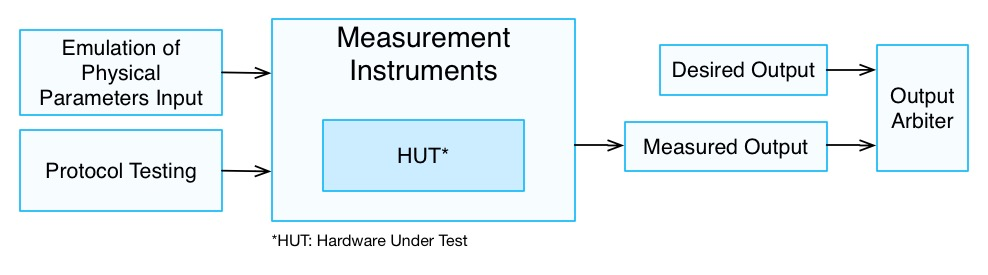
\includegraphics[scale=0.45]{immagini/Testing_Gridsense_TestSystem}
% \caption{Testing System} 
% \label{fig: Testing_Gridsense_TestSystem}
%\end{center}
%\end{figure}



\begin{enumerate}
  \item \textbf{Learn what is a stepper motor:}  (half day)
  	\subitem Student must do a small research of what is a stepper motor.
  	\subitem description of the kinds of steppers (Unipolar - Bipolar).
  \item \textbf{Learn how to use a stepper motor:} (half day)
  	\subitem Student must make a small research of how to control the two kind’s of motors and learn the sequences for each stepper.
  	\subitem Student must identify the HW needed to connect the Stepper to the Arduino. (use of LM293/LM293D)
  \item \textbf{Programming the sequence using Arduino:} (one day)
  	\subitem Using PINx of the Arduino's API
  		\subsubitem Stepper in clockwise way direction
  		\subsubitem Stepper in counter clockwise way direction
  		\subsubitem Stepper in both directions
  	\subitem Using the PORTx of the microcontroller
  		\subsubitem Stepper in clockwise way direction
  		\subsubitem Stepper in counter clockwise way direction
  		\subsubitem Stepper in both directions
  \item \textbf{Optimise the program Part 1} (one day)
	\subitem Understand the use of push buttons using Arduino
		\subsubitem Identify the bouncing effect
		\subsubitem solve the problem using "anti-bouncing" techniques
  	\subitem Add the use of push buttons to define the direction of the stepper motor (left and right).
  	\subitem Add the use of push buttons to set the velocity of the stepper motor
  \item \textbf{Optimise the program Part 2} (one day)
  	\subitem Introduce sensors to identify the position of the motor.
  	\subitem \textcolor{red}{MORE IDEAS TO ADD HERE}


\end{enumerate}
